\documentclass[]{article}
\usepackage{graphicx}
\usepackage[a4paper,margin=1in,footskip=0.25in]{geometry}
\usepackage{float}
\usepackage[parfill]{parskip}
\graphicspath{ {./images/} }
\usepackage{subcaption}
\usepackage[ruled,vlined]{algorithm2e}

%opening
\title{Implementing Q-Learning for Path Finding}
\author{Ben Hynes}

\begin{document}
	
\maketitle

\begin{figure}[H]
	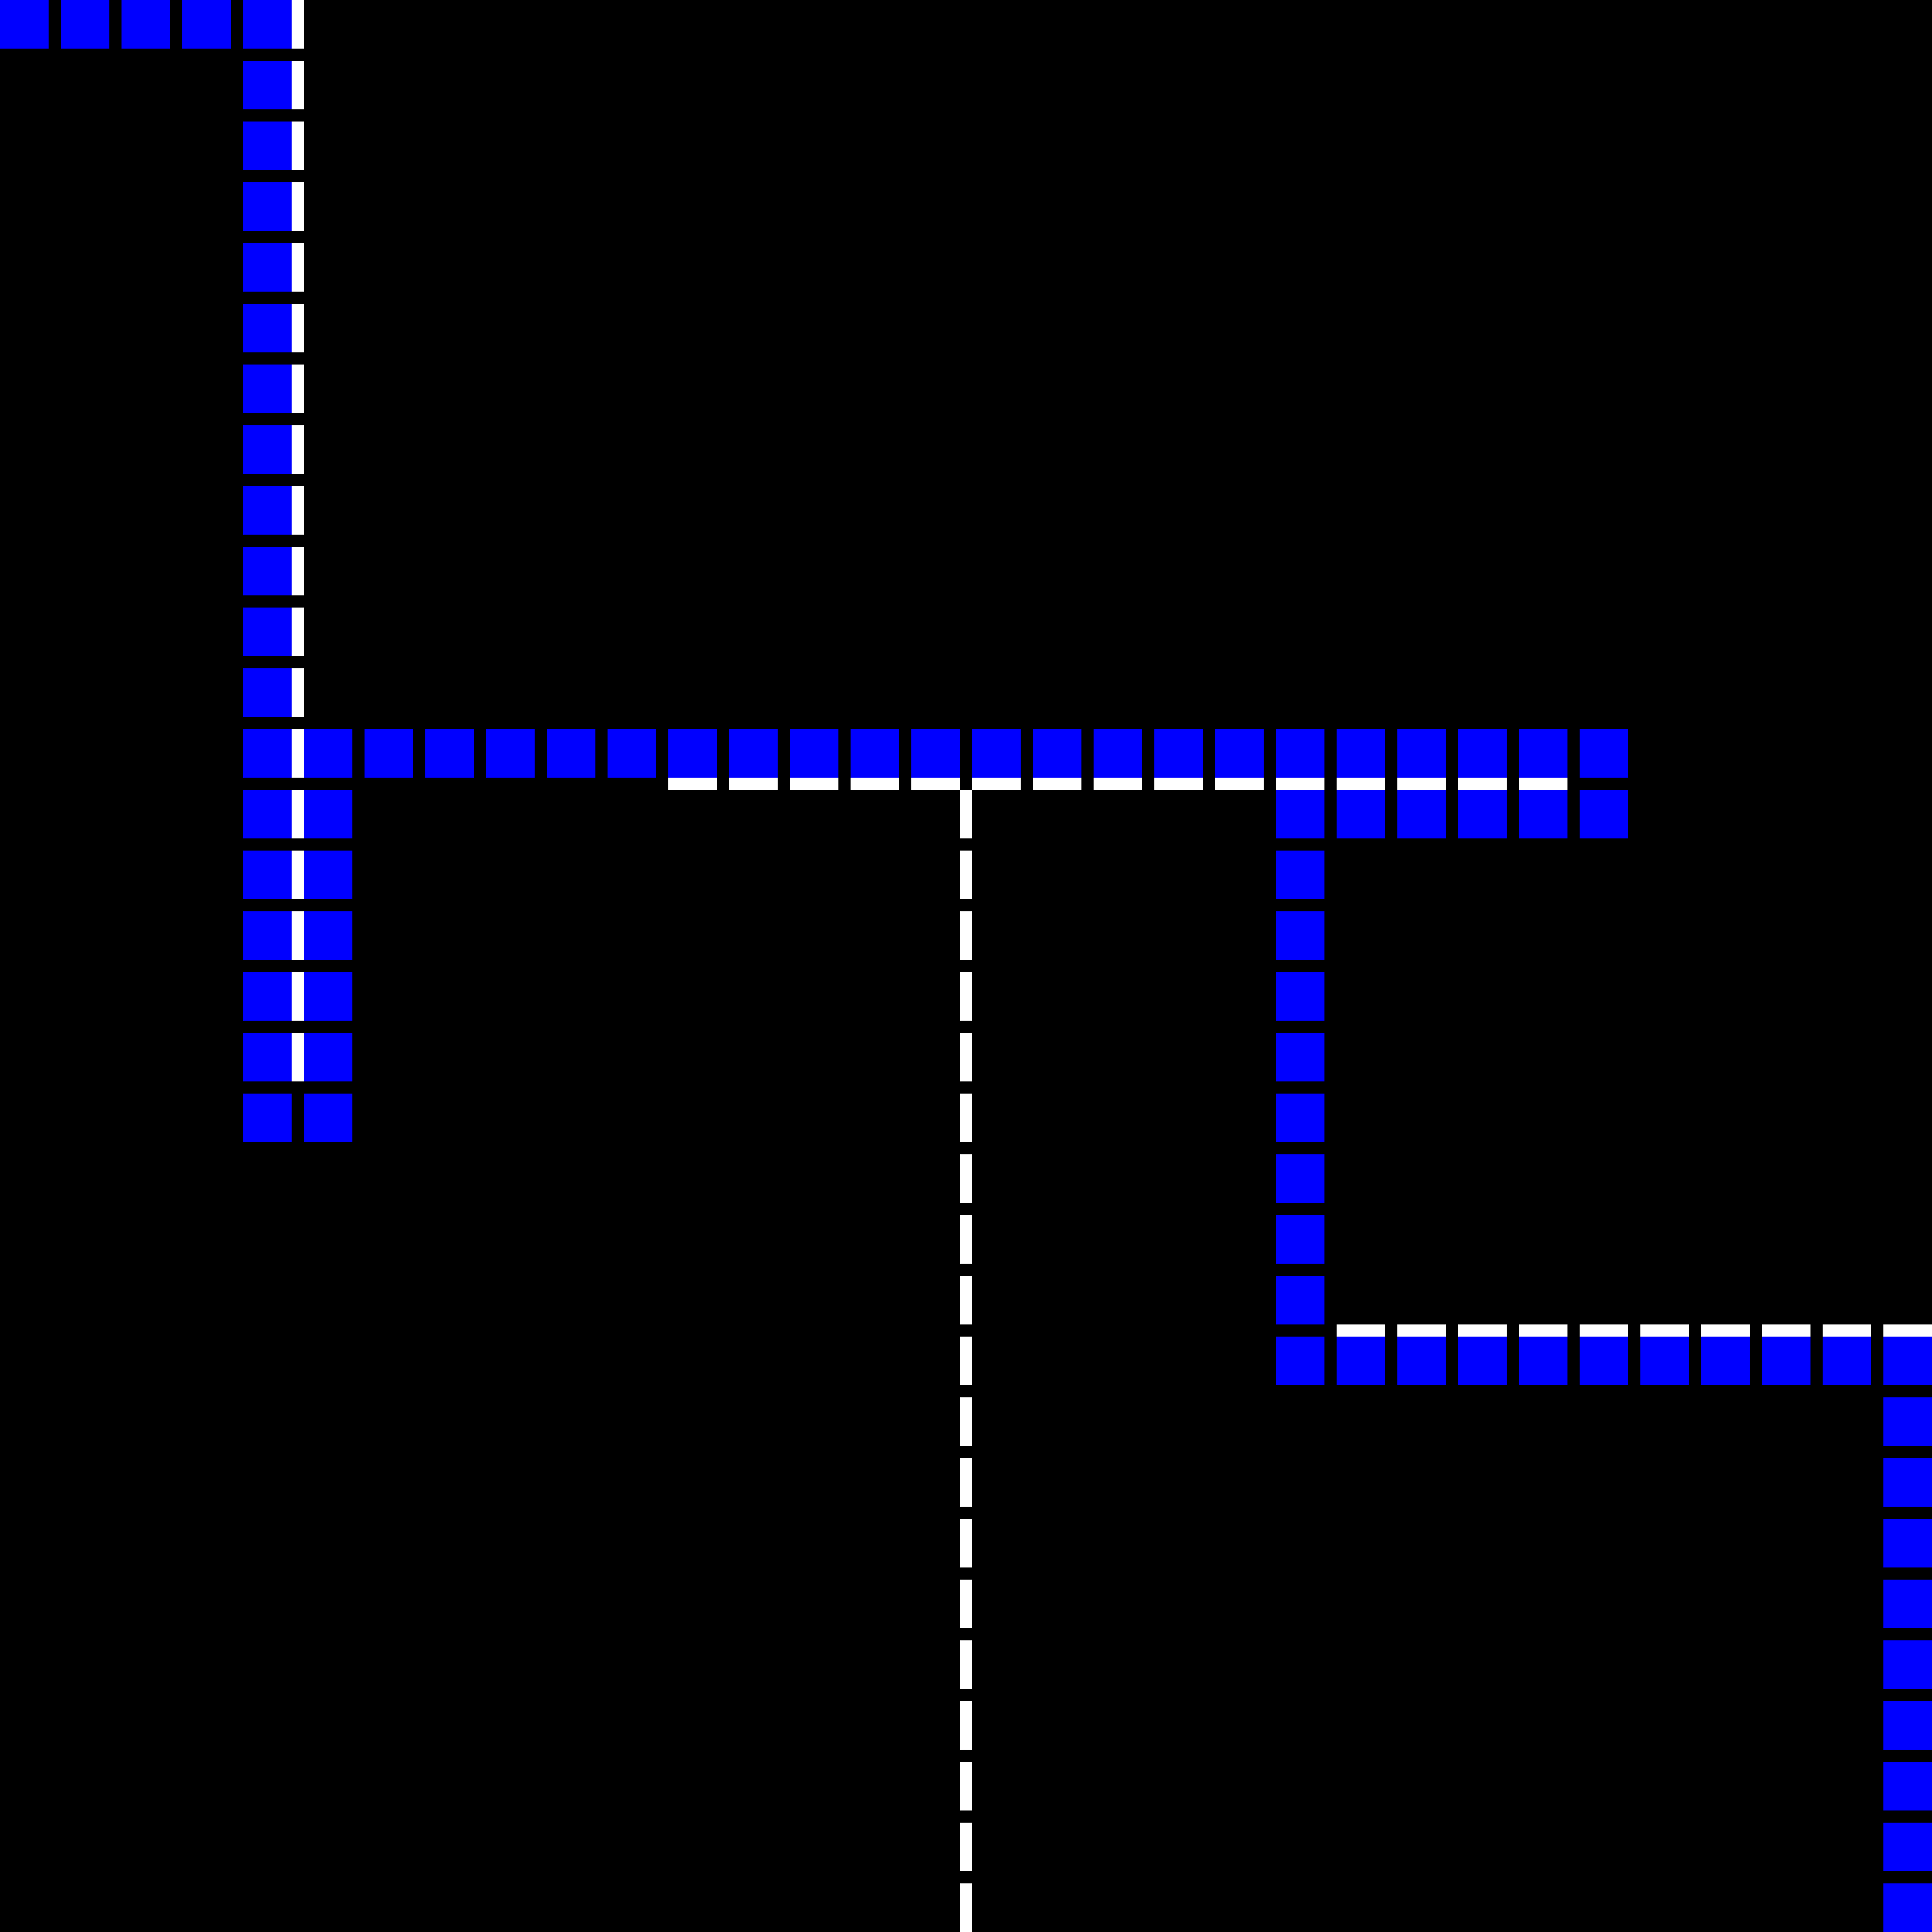
\includegraphics[scale=0.05]{1ma}
	\centering
	\caption{Final Q-Learn route.}
\end{figure}

\clearpage

\section{Introduction}

\subsection{Markov Decision Process}

A Markov chain is a stochastic model meaning that it is a process that involves randomness. It is uncertain which state will come after the current state. The chain describes a sequence of possible events in which the probability of each event depends only on the state attained in the previous event. 

\begin{figure}[H]
	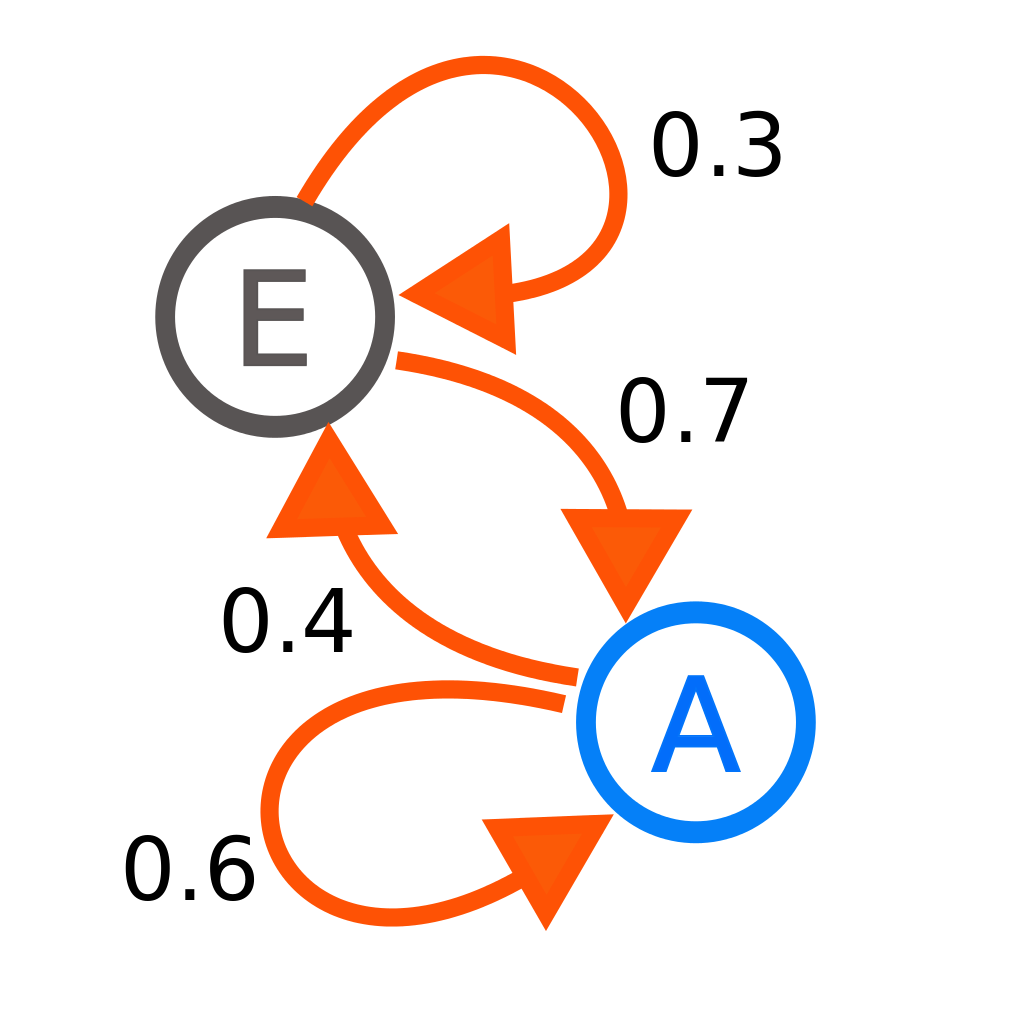
\includegraphics[scale=0.13]{markov}
	\centering
	\caption{A two-state Markov process.}
\end{figure}

A Markov decision process is a discrete time stochastic control process. Markov decision processes provide a mathematical framework for modelling decision making in situations where outcomes are partly random and partly under the control of a decision maker. A stochastic process has the Markov property if the conditional probability distribution of future states of the process depends only upon the present state, not on the sequence of events that preceded it. A process with this property is called a Markov process.

At each time step, the process is in some state $s$ and the decision maker may choose any action $a$ that is available in state $s$. The process responds at the next time step by randomly moving into a new state $s'$ and giving the decision maker's a corresponding reward $R_a(s, s')$.

The probability that the process moves into its new state $s'$ is influenced by the chosen action. It is given by the state transition function $P_a(s, s')$. The next state $s'$ depends on the current state $s$ and the decision maker's action $a$. But given $s$ and $a$, it is conditionally independent of all previous states and actions and therefore satisfies the Markov property. 

\begin{figure}[H]
	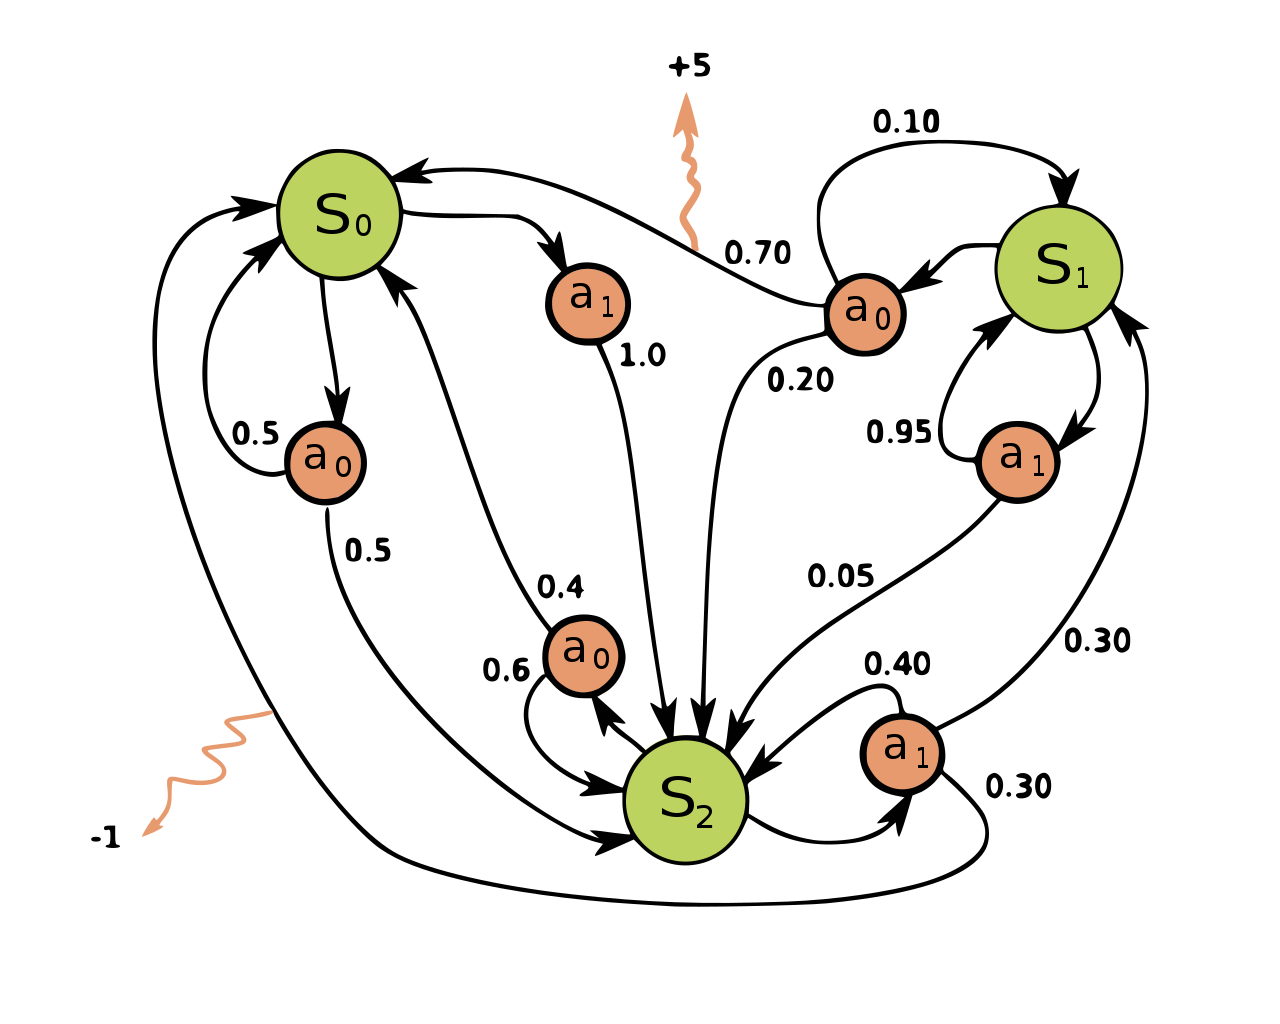
\includegraphics[scale=0.20]{mdp}
	\centering
	\caption{A Markov Decision Process with rewards in orange.}
\end{figure}

\subsection{Q-Learning}

Q-learning is a model free reinforcement algorithm. Model free means that it does not have access to a transition probability distribution associated with the MDP as this is what we aim to find. In q-learning, there is one q value for each possible action you could take from each state.

\[Q^{new}(s_t,a_t) = Q(s_t,a_t)+\alpha(r_t+\gamma \; max \, Q(s_{t+1},a) - Q(s_t,a_t))  \]

where 
\begin{itemize}
	\itemsep-0.4em 
	\item $Q^{new}(s_t,a_t)$ is the new Q value
	\item $Q(s_t,a_t)$ is the old Q value
	\item $\alpha$ is the learning rate
	\item $r_t$ is the reward function
	\item $\gamma$ is the discount factor
	\item $max \, Q(s_{t+1},a)$ is the estimation of future value
	
\end{itemize}

\section{Implementation}

This implementation is fully scalable, having been tested up to 32x32 pixel image sizes. In a 32x32 grid there are 1,024 states and 1,024 actions, totalling 1,048,576 state-action pairs. A reward of 1 will be given to the agent if a state is directly reachable from the current state. The destination state will have a reward of 999. All other state-action pairs have a reward of 0. The algorithm for training the agent and calculating the Q table can be seen below.

\begin{algorithm}[H]

	\SetAlgoLined

	
	\For{N}
	{
		set $s$ to random state\;
		\For{each $a$ from $s$}
		{
			\If{$r_{s,a}>0$}
			{
				add to list of playable actions\;
			}
			set $s_{t+1}$ to state from random action choice\;
			calculate temporal difference\;
			update q value for $s_t, a_t$\;
		
		}
	}

	\caption{Updating Q values}

\end{algorithm}


\section{Results}

Finding a balance between exploration and exploitation can be difficult. Several tests were run for various values of $N$, the number of training moves the agent makes. The graphs on the right show the rate of learning (specifically, the average temporal difference) as these training moves are made. This decreases over time as the agent learn about the environment.

\clearpage

\begin{figure}[ht]
	\centering
	\begin{minipage}[c]{0.3\linewidth}
		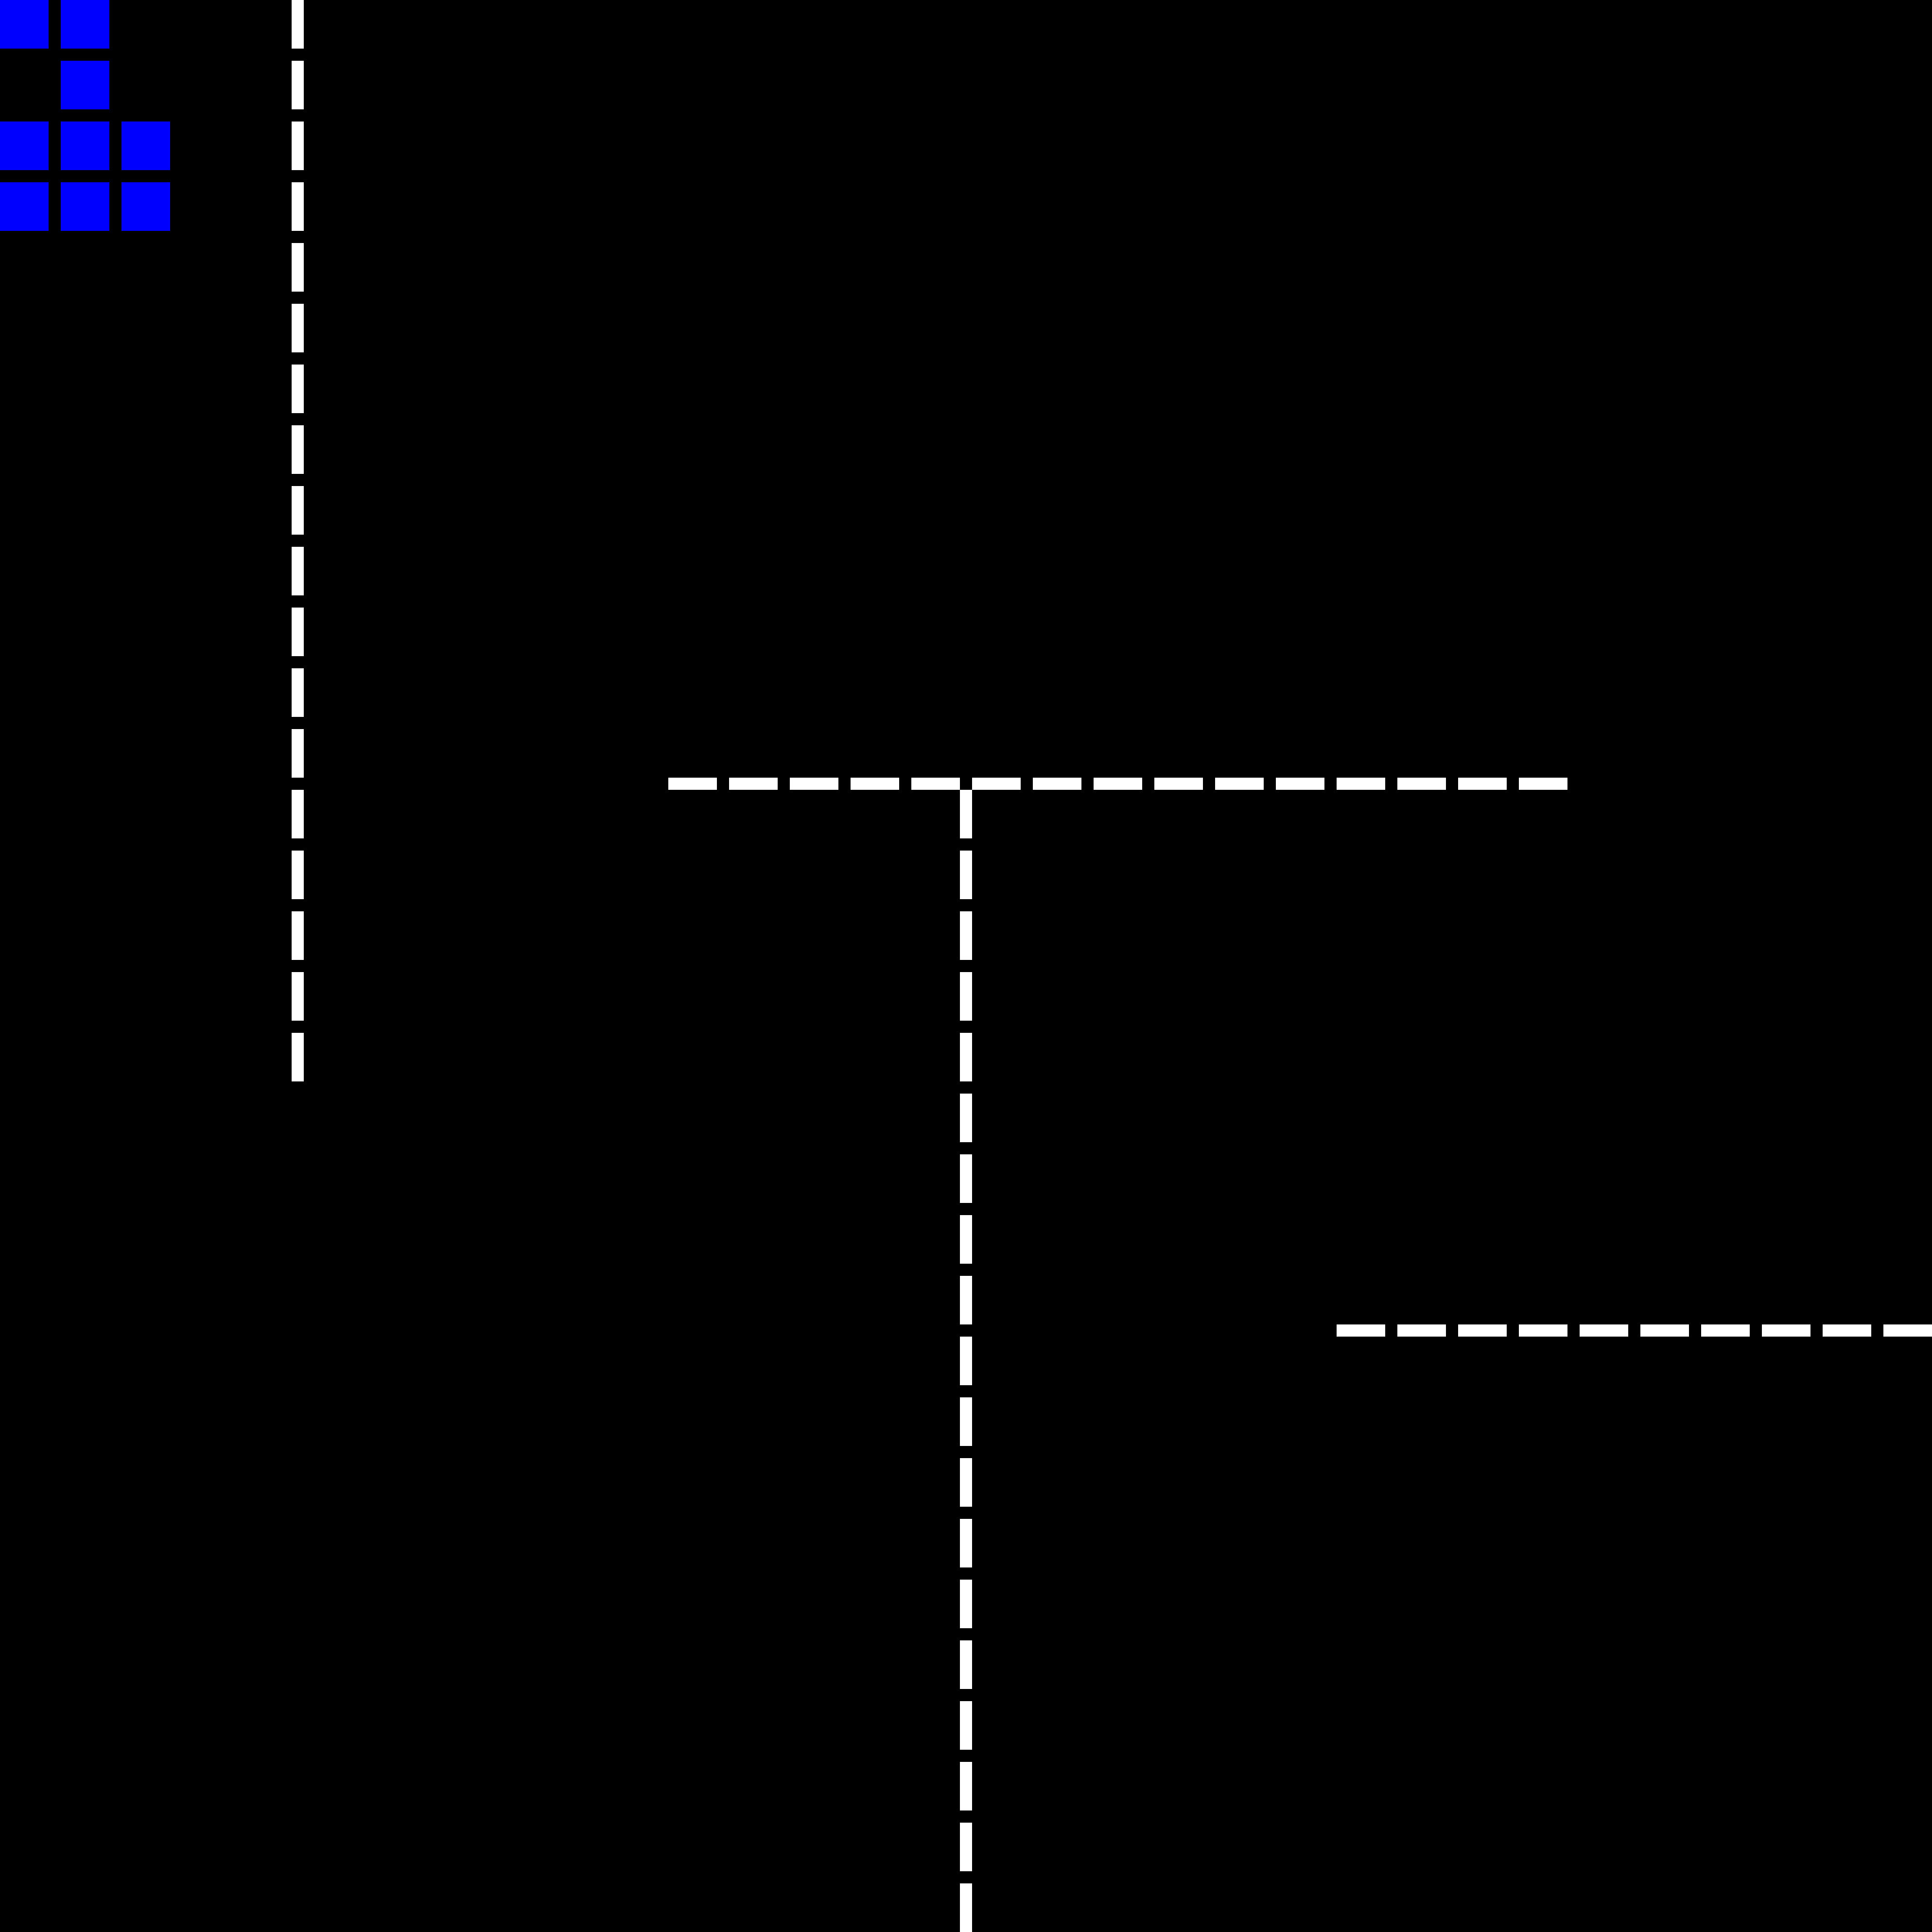
\includegraphics[width=4.5cm]{100kb}
		\caption{N = 100K}
	\end{minipage}
	\quad
	\begin{minipage}[c]{0.45\linewidth}
		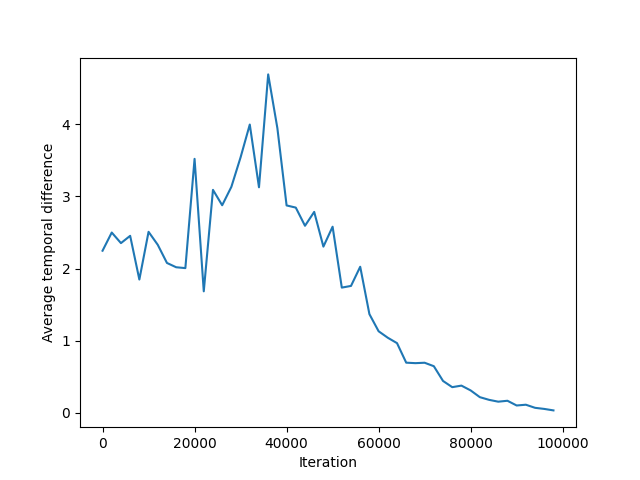
\includegraphics[width=6.5cm]{100ka}
		\caption{Average temporal difference}
	\end{minipage}
\end{figure}

Increasing $N$ to 100k allows the agent to find an optimum path.

\begin{figure}[ht]
	\centering
	\begin{minipage}[c]{0.3\linewidth}
		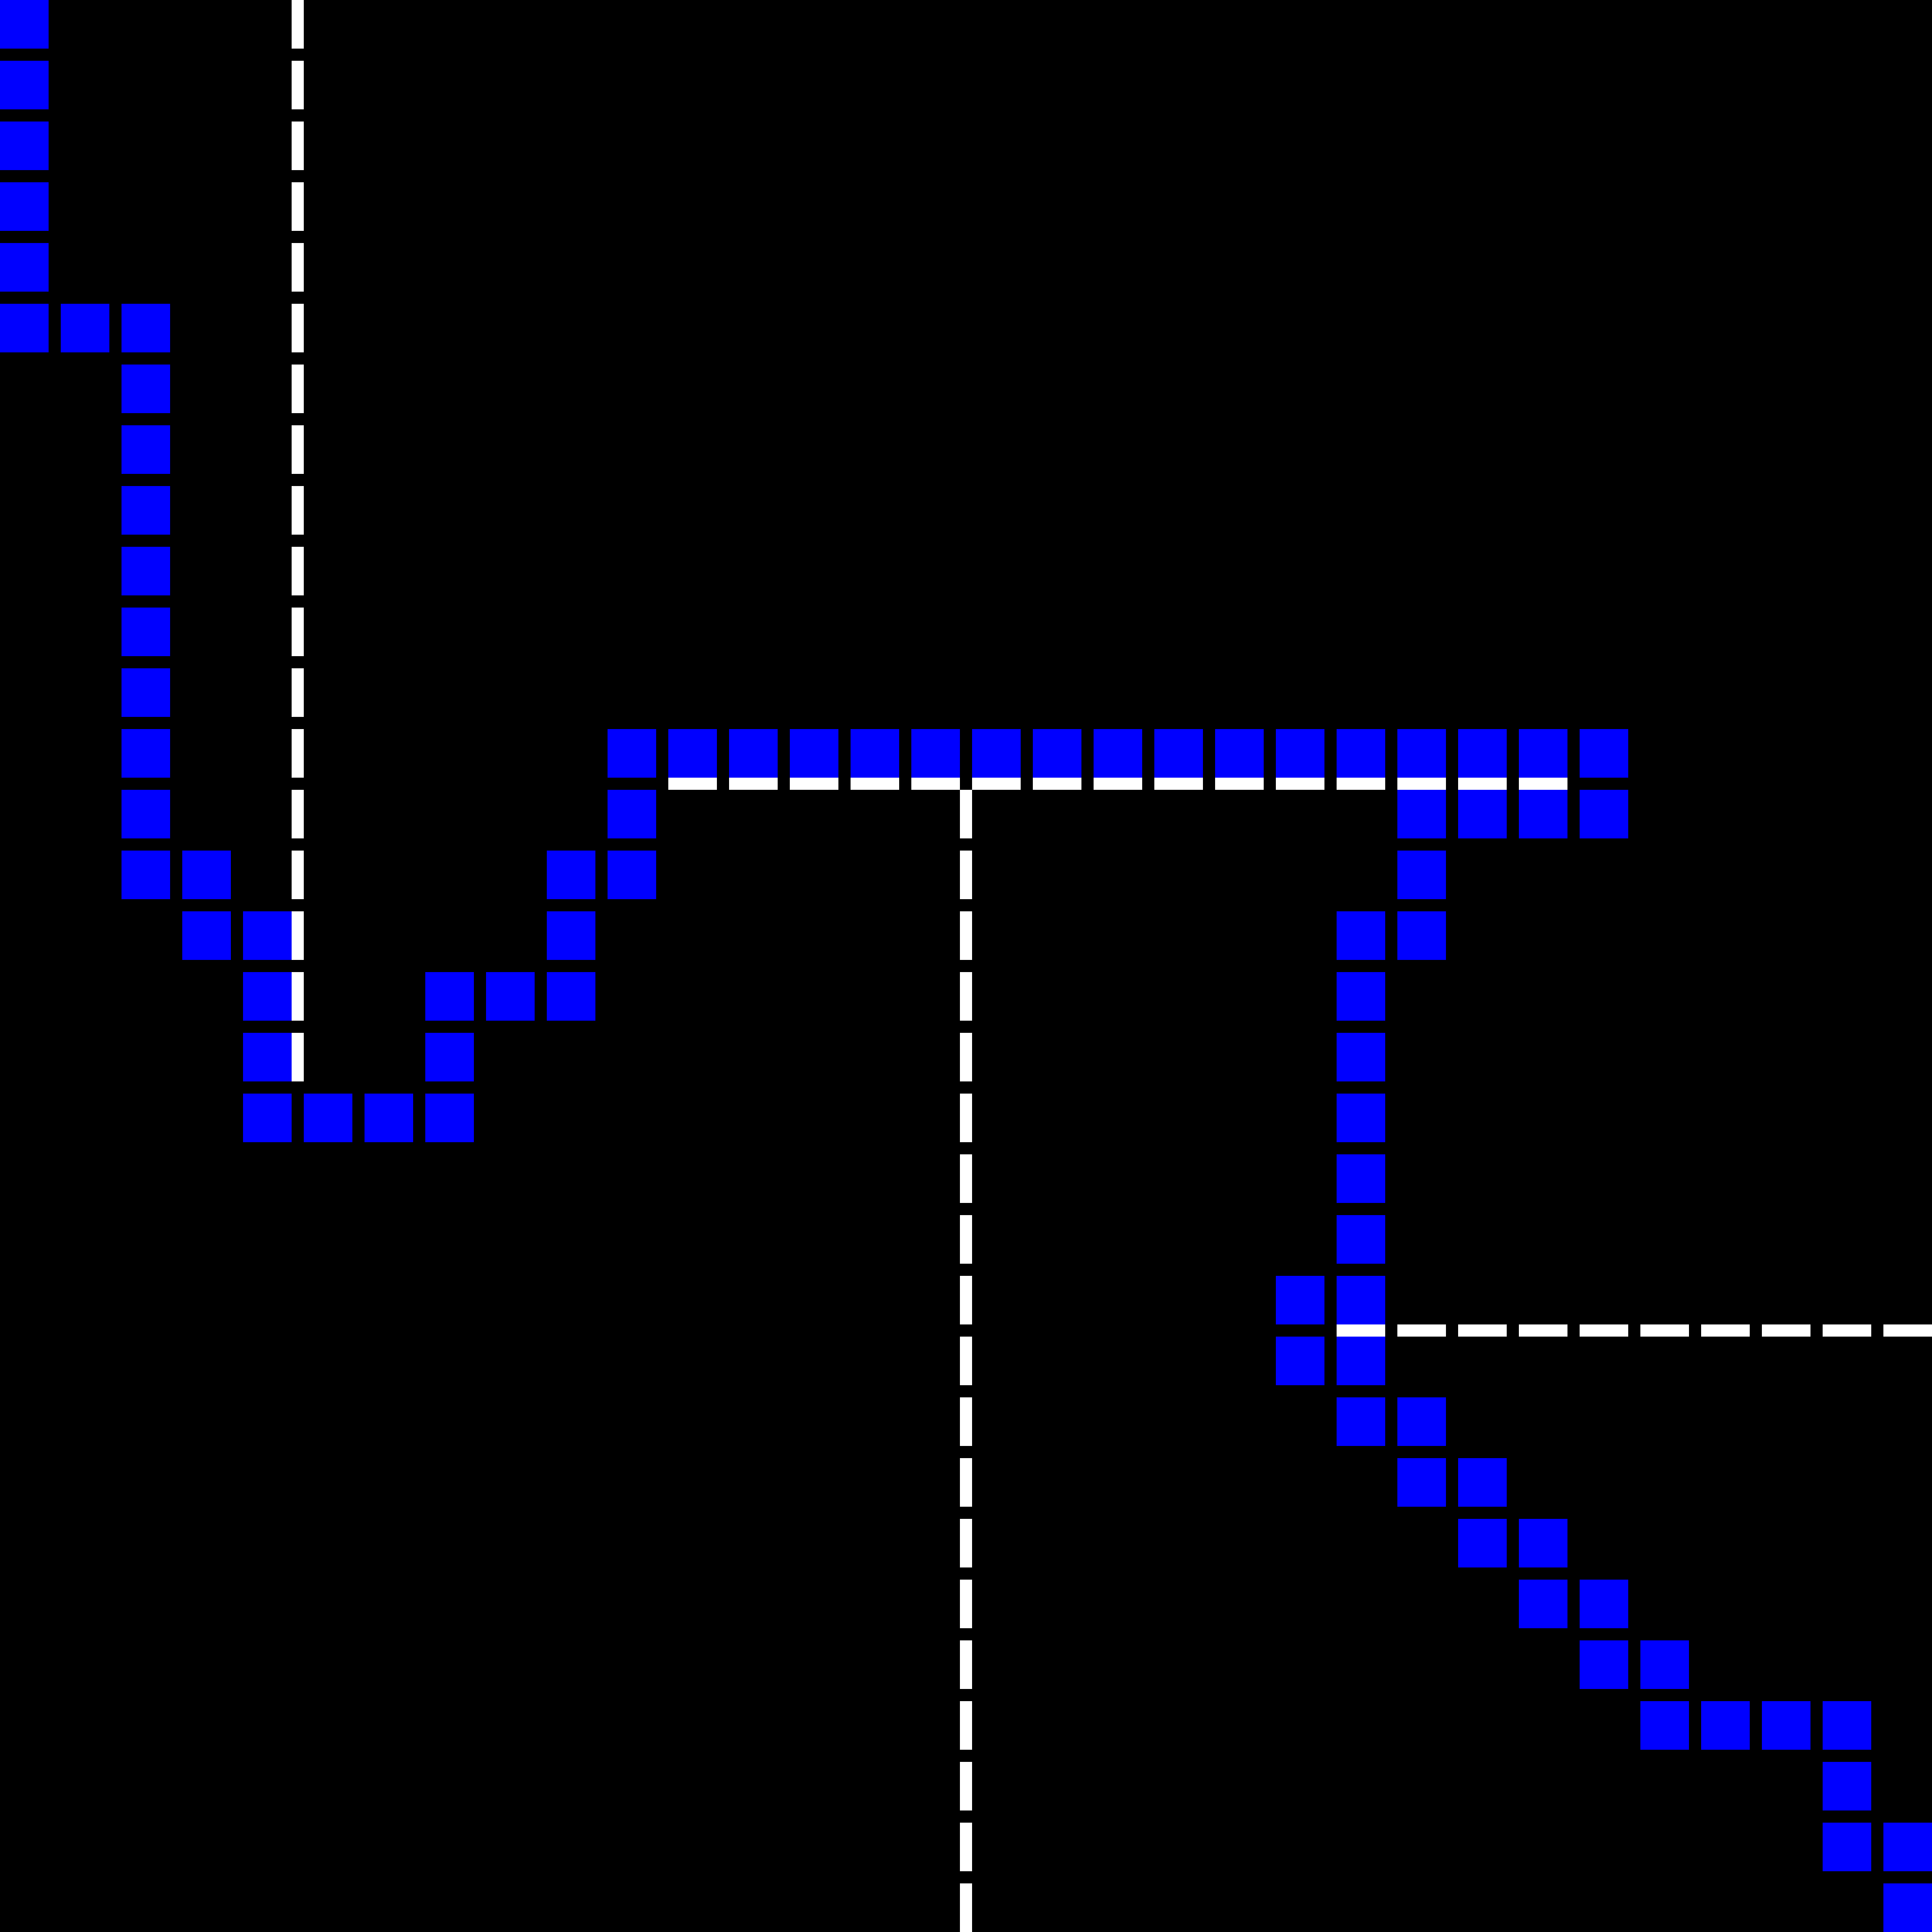
\includegraphics[width=4.5cm]{250kb}
		\caption{N = 250K}
	\end{minipage}
\quad
\begin{minipage}[c]{0.45\linewidth}
	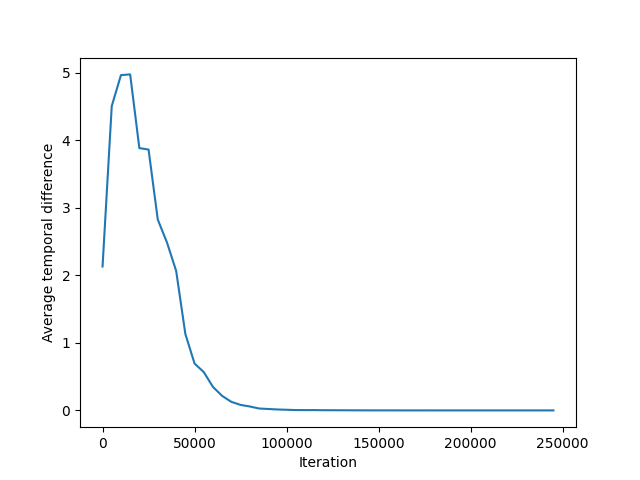
\includegraphics[width=6.5cm]{250ka}
	\caption{Average temporal difference}
\end{minipage}
\end{figure}

Interestingly, although the agent has found the shortest route, further training it will cause it do suggest a route with the minimum number of turns. 

\begin{figure}[ht]
	\centering
	\begin{minipage}[c]{0.3\linewidth}
		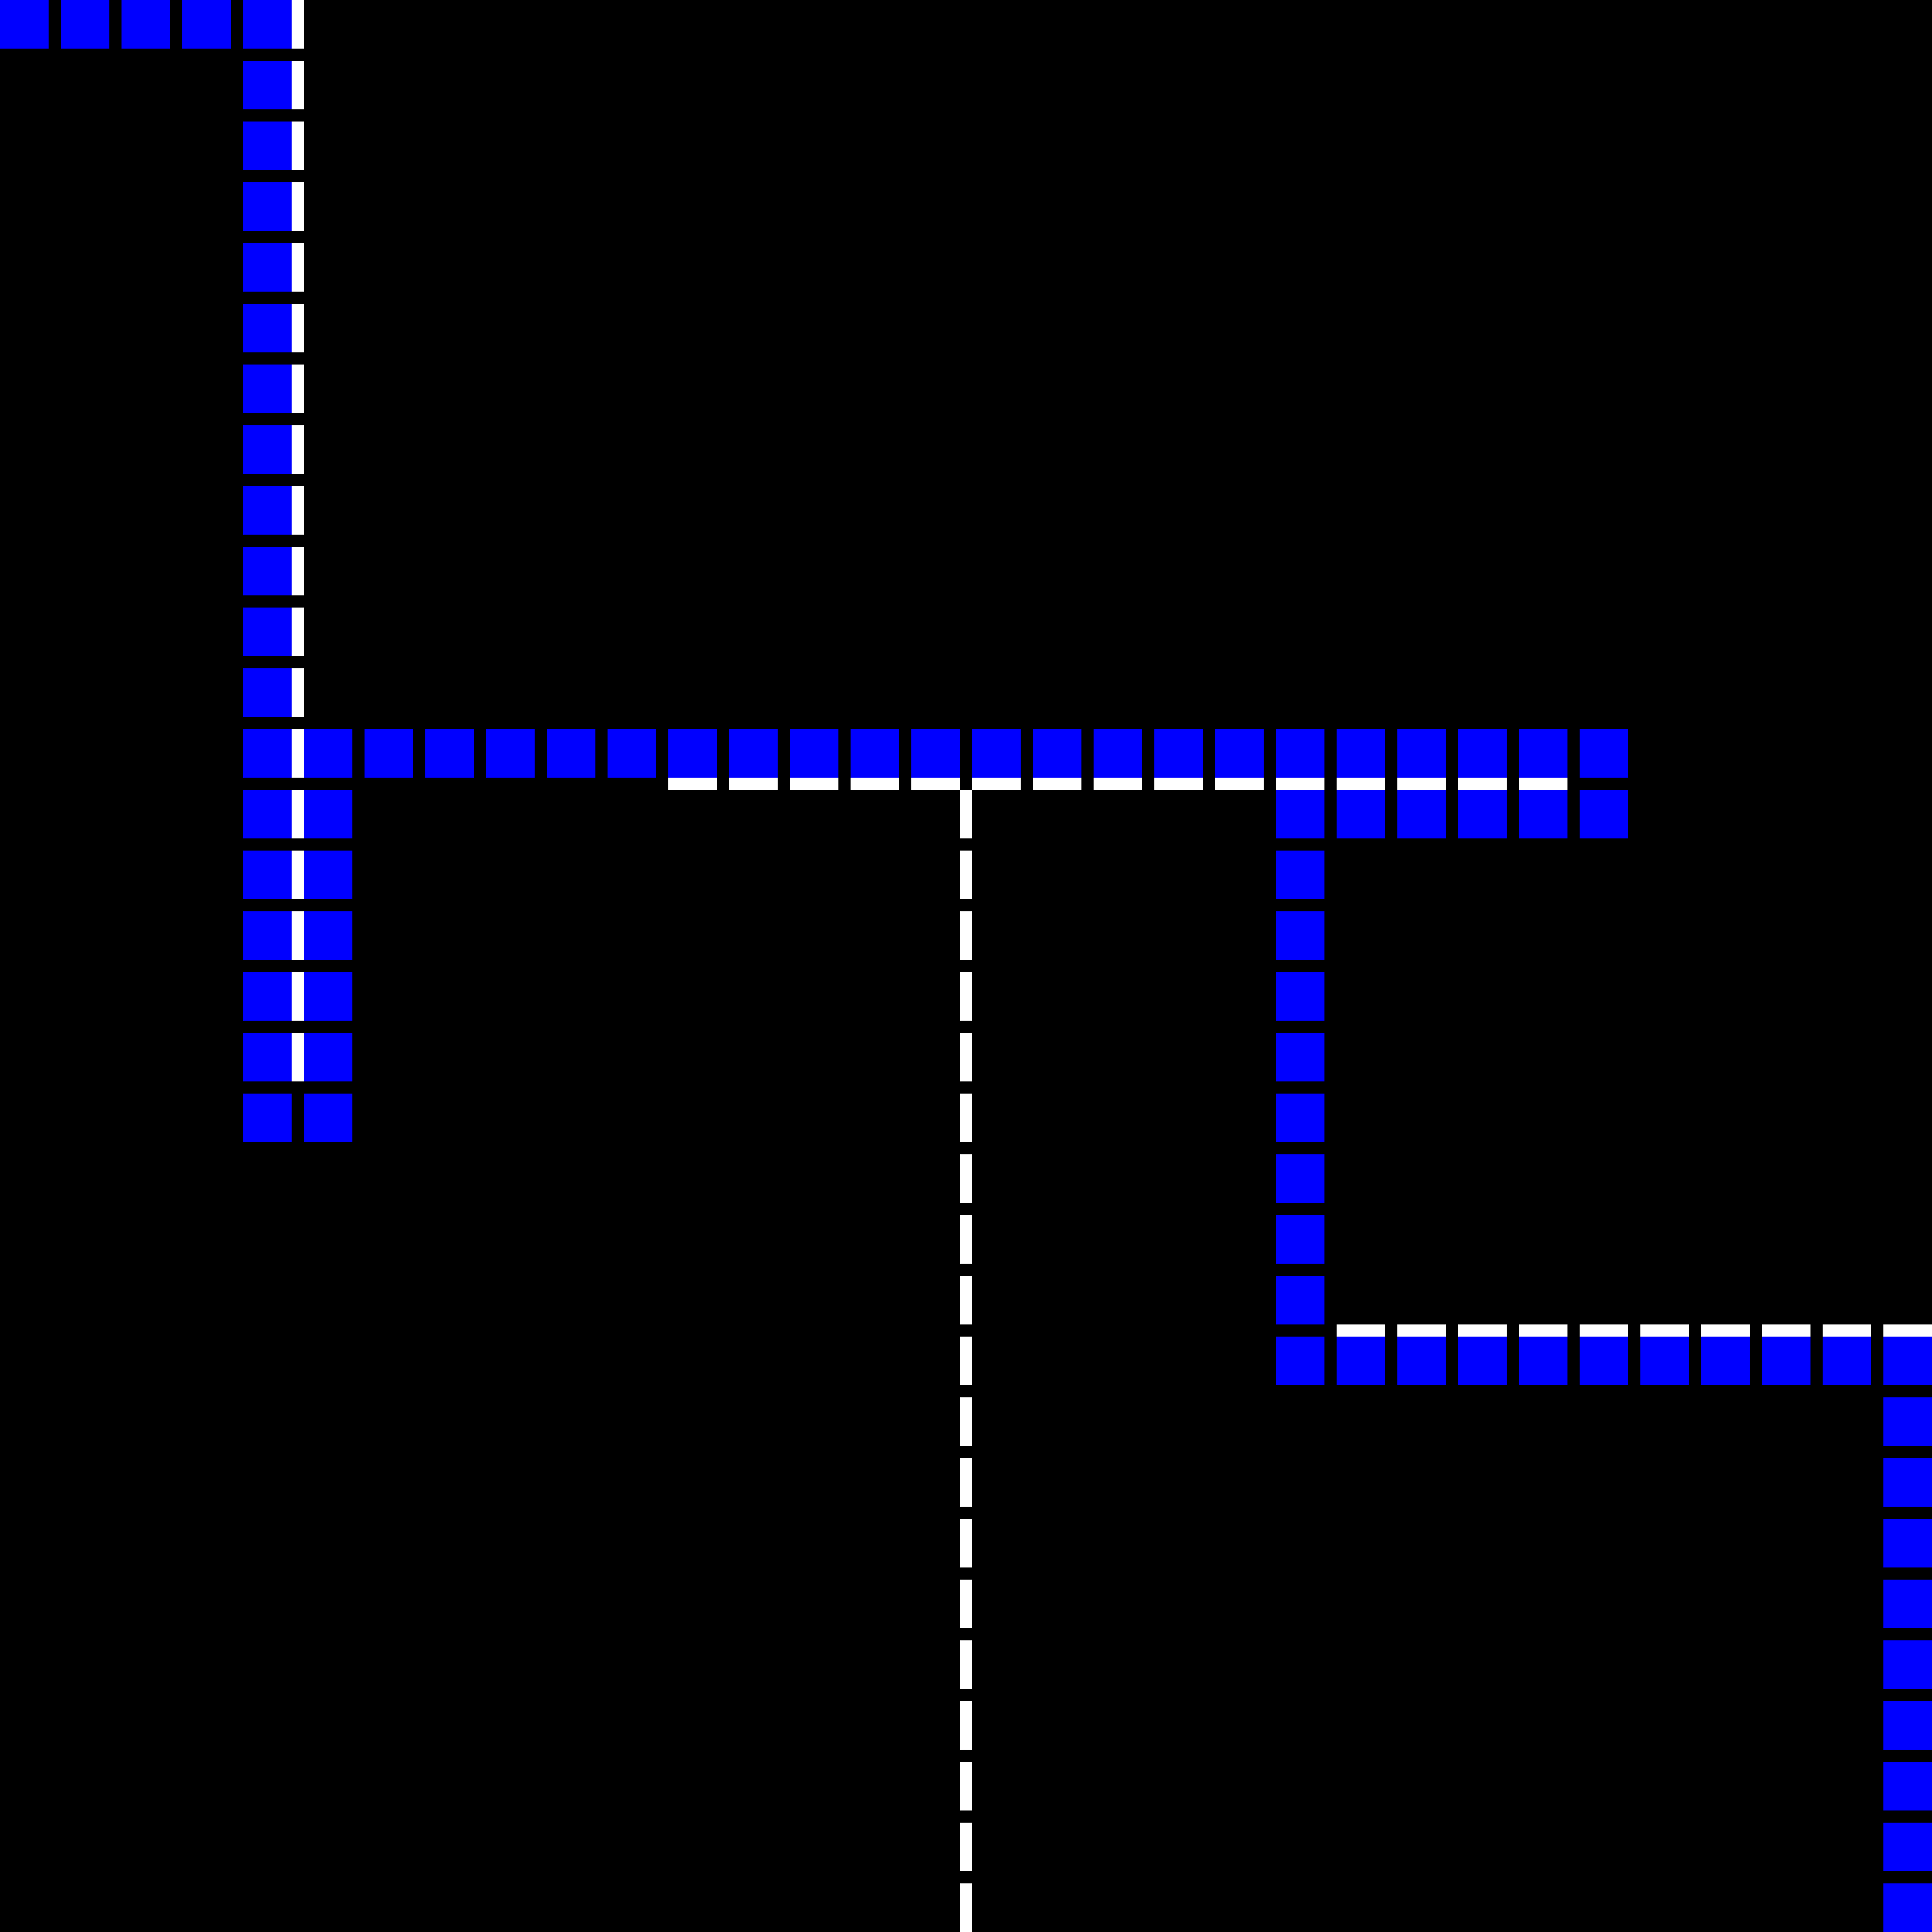
\includegraphics[width=4.5cm]{1ma}
		\caption{N = 1M}
	\end{minipage}
	\quad
	\begin{minipage}[c]{0.45\linewidth}
		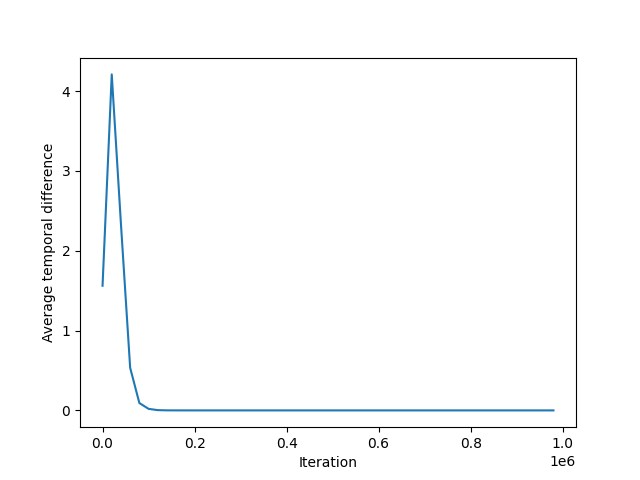
\includegraphics[width=6.5cm]{1mb}
		\caption{Average temporal difference}
	\end{minipage}
\end{figure}


\end{document}